
\documentclass[12pt]{article}

\usepackage{newtxtext,newtxmath}
\usepackage{graphicx}
\usepackage{float}
\usepackage[letterpaper,margin=1in]{geometry}

\linespread{1.5}
\frenchspacing

\renewenvironment{abstract}
	{\quotation}
	{\endquotation}

\date{}

\renewcommand\refname{References and Notes}

\makeatletter
\renewcommand{\fnum@figure}{\textbf{Figure \thefigure}}
\renewcommand{\fnum@table}{\textbf{Table \thetable}}
\makeatother

\usepackage{scicite}

\usepackage{url}

\usepackage[backend=bibtex,style=ieee]{biblatex}
\addbibresource{references.bib}  

\newcommand{\pcc}{\,cm$^{-3}$}	

\def\scititle{
	Tenure Systems and the Global North vs South vs East : A Comparative Analysis of the Applicability of Gentrification outside the Anglo-American context
}
\title{\bfseries \boldmath \scititle}

\author{Keina Ga\\Institute for Computing in Research}

\begin{document} 

\maketitle

\begin{abstract} \bfseries \boldmath
This study, with its focus on the phenomena of global gentrification, quantifies regional variances in gentrification mechanisms and effects. Comparative case studies of New York City and Singapore demonstrate how cities’ different tenure systems result in varied effects of two main gentrification mechanisms, market-driven and tenure conversion. The findings of a literature analysis on articles from the Global North, Global South, and Global East demonstrate how attributed gentrification mechanisms differ across global regions. This study found gentrification to be context specific and dependent, thus unable to be generalized to narrow frameworks, such as an Anglo-American framework. This exploration of cross-regional gentrification emphasizes the need to establish and apply a broader framework for the study of global gentrification to account for regional variance.
\end{abstract}

\section*{1 Intro}
\subsection*{1.1 Background, objectives, and hypothesis} 
The purpose of this study is to observe and quantify differences in the effects of varied mechanisms of gentrification in the setting of various global regions. The central research question is whether the causes and effects of gentrification are regionally dependent or if they are applicable outside the Anglo-American context. \\

Gentrification occurs when wealthier people move into lower income neighborhoods and displace long time residents by increasing housing and rent prices. In this study, the definition of gentrification is broadened to embody an urban process where changes in housing and land lead to displacement of residents. The study also involves an Anglo-American context for comparison, a context regarding the socio-economic framework of the Global North and market-driven gentrification mechanisms. An Anglo-American focus is fabricated out of the assumption that America is the epitome of classic gentrification of rising housing and rent prices displace residents due to the country’s unregulated and competitive housing market. However, an Anglo-American version of gentrification is limited in global application. [1] \\ 

The pretense of this study is that the process of gentrification is globalized. International cities are upgrading economically and stylistically which in turn changes their housing scenes. When studying gentrification on a global scale, regionally dependent factors such as tenure systems, local history, and economic conditions must be considered. This study highlights that gentrification is a global but geographically uneven process. [2] \\ 

The two mechanisms of gentrification of focus are 1) Market-driven displacement in private competitive tenure systems where residents are priced out of housing due to an increase in rent gap - the financial difference between a property's actual rental income and its higher income potential. This mechanism is driven by capitalism and is the standardized explanation of the cause of gentrification. 2) Tenure-conversion displacement in predominantly state owned tenure systems where residents are displaced due to the privatization and dispossession of public, and occasionally untitled, housing. This form of gentrification is incited by state regulations and redevelopments. [3] \\ 

To observe both differences of tenure systems and different socio-economic frameworks, the Global North, Global South, and Global East, the study is broken down into two parts 1) a quantitative pattern analysis of case studies of two cities, New York City with its market-driven tenure system and Singapore with its state-dominated tenure system. 2) A comparative literature analysis of articles from the Global North and Global South and Global East. \\

The hypothesis is that comparisons of cities with different tenure systems and comparisons of regions with different socio-economic frameworks will exhibit diversity in the identified mechanisms of gentrification.
\\

\subsection*{1.2 Contextualizing the differences of the Global North, Global South, Global East} 
The Global North includes the United States, United Kingdom, Western Europe, Australia, and Canada. Land in the Global North is predominantly titled and privately owned. These countries are driven by large real estate industries and follow a capitalistic framework that makes it easy for individual agents to exploit the housing market by inflating land value at the presented opportunity of a rent gap. The cause of gentrification in the Global North is redevelopments of inner-city working neighborhoods to accommodate middle and upper class residents, extreme increases in rent prices by landlords, condo conversions, as well as tourism driven upgrading of short term rentals such as Airbnbs. [4] [5] \\ 

The Global South includes much of Africa, Latin America and some parts of Asia. These developing countries tend to have weak governments and legal enforcement of tenure due to legacies of colonialism. Land in the Global East is a mix of private property and state-ownership, while much of it untitled and informal, such as slums or squatter settlements. The state occasionally invokes forced formalization and redevelopment of informal settlements which results in the displacement of large communities. The cause of gentrification in the Global South is the commodification of housing and large scale slum evictions. [6] [7] \\ 

The Global East includes China, Japan, South Korea, and Russia. These countries are wealthy and developed, with China and Russia bearing histories of socialism. Land in the Global East is predominantly owned and regulated by the state, with housing units privately owned. The state facilitates property demolitions and upgrades of land and the leasing of property. These countries are driven by state-led initiatives, but also exhibit some market-driven aspects of private acquisitions. The cause of gentrification in the Global East is dispossession in the inner-city, displacement of long-term residents to the urban periphery to create new apartments for the wealthy, and conversion of districts into upscale city quarters. [8] [9] \\

\section*{2 Methodology}
\subsection*{2.1 Comparative case studies of New York City and Singapore} 
The comparative analysis of tenure systems involves two case studies New York City - representative of a city of high-value private-unregulated real estate and a competitive housing market - and Singapore - representative of a city wherein land is predominantly owned by the state that regulates developments, acquisitions, and sales. Per each city, three areas are selected, an area 1) to serve as a control 2) that experienced rent-gap market-driven displacement of residents 3) that experienced tenure conversion where public lands were privatized. For the specific areas, to ensure similarity in the scale of residential population sizes between the cities, New York City’s case studies are three neighborhoods and Singapore’s case studies are three classified planning areas/residential towns. \\

For New York City, the following neighborhood zip codes were selected:\\
West Village of Greenwich Village (10014) - regarded as a protected historic district by the Landmarks Preservation Commission (LPC) with heavy regulation of new housing repairs and construction \\
Bedford-Stuyvesant and Crown Heights (BS and CH) of Brooklyn (11216) - BS and CH underwent extreme increases in median home rent compared to the rates of Brooklyn and the general New York City due to landlords raising prices for prime estate \\
Ocean Bay and Far Rockaway (OB and FR) of Queens (11691) -  OB and FR underwent renovations of many of its housing complexes due to financial investments from the city and much funding from private developers and investors, which led to newfound private management of housing \\

For Singapore, the following planning area sector codes were selected: \\
Ang Mo Kio (56, 57) - deemed by Urban Redevelopment Authority (URA) to house many conservation areas and thus has new housing repairs and construction heavily regulated \\
Bukit Merah (14, 15, 16) - underwent extreme increases in rent costs due to the working-class neighborhood having undergone rapid housing development and upgrading of urban amenities \\
Geylang (38, 39, 40, 41) - experienced state-led urban housing renewal, by the Singapore government and its Housing Development Board (HDB), with some lands taken up by the state to be leased and sold for commercial development, thus leading to the relocation and displacement of many residents \\

These six areas, three from New York City and three from Singapore, are observed through the unit of analysis of median household income and residential population (with data collected from each nation’s census studies). These two units of analysis are charted in terms of percent change from 2010 to 2020. \\

\subsection*{2.2 Literature analysis of Global North vs South vs East} 
The literature analysis is conducted through a socio-economic framework of the three regions, the Global North, Global South, and Global East. \\

Ten academic journal articles are selected per each global region. Two banks of keywords are assembled to embody the themes of 1) Market-driven gentrification and 2) Tenure-conversion gentrification: \\

key\_market = ["rent gap", "rent-gap", "private renovation", "upgrad", "mortgage lend", "rent", "tourism", "airbnb", "luxury", "real estate", "speculat", "land value", "flip", "landlord", "private capital", "private equity", "venture capital", "return on investment", "market rate", "migra", "disinvest", "reinvest"] \\

key\_tenure = ["state led", "state-led", "city led", "public housing", "demoli", "relocat", "dispossess", "commodif", "regenerat", "slum clearance", "tenure reform", "renew", "expropriat", "resettle", "municipal", "decant", "permanent hous", "temporary hous", "state polic"] \\

Three sets of ten articles are run through a model that quantifies the frequency of each keyword from both theme banks. The model breaks down the files into a parsable format. The model then uses a threshold to discern the theme of the articles if a keyword should be found in the article more than two times: \\

\begin{figure}[H] 
	\centering
	\includegraphics[width=1.0\textwidth]{SC1.png}
    \caption{\textbf{Code section 1} Code that counts the number of keywords that appear per article: num\_market is the total count of keywords found in the bank of keywords that classifies market-driven gentrification. key\_phrase is the variable to represent a word of the list of keywords key\_market. num\_tenure is the total count of keywords found in the bank of keywords that classifies tenure conversion gentrification. key\_phrase is the variable to represent a word of the list of keywords key\_tenure. temparticle is the current article that gets parsed.}
\end{figure}

If a keyword is found, the count is stored in a dictionary pertaining to the specific article. The requirements of thematic classification with X as the variable for the count of keywords found: \\

1) Market-driven gentrification: Minimum 4 / 22 keywords (X $>$ 3 / 22) \\
2) Tenure conversion gentrification: Minimum 3 / 19 keywords (X $>$ 2 / 19) \\

\begin{figure}[H]
	\centering
	\includegraphics[width=0.5\textwidth]{SC2.png}
    \caption{\textbf{Code section 2} Code that determines mechanisms of gentrification per article}
\end{figure}

Prints “yes” or “no” per each theme of market-driven gentrification and tenure conversion gentrification based on the threshold count of keywords.\\

\subsection*{2.2 Calculating statistical significance: Kruskal-Wallis test} 
Both data from part 1) Median household income and residential population from 2010 to 2020 of areas in New York City Singapore and part 2) Attributed gentrification mechanisms of articles on the Global North vs South vs East, are analyzed with a Kruskal-Wallis statistical test to determine the significance of results. \\

The Kruskal-Wallis test is a method used to compare independent groups to see if their medians or distributions differ. It is used in this study to prove statistical significance in differences between groups, as well as variance of data. \\

The Kruskal-Wallis test evaluates differences in rank medians by combining the assigned ranks of data (ranked from lowest to highest 1 ~ N, the total number of data points) to calculate the H-value: \\

\begin{equation}
	H = \frac{12}{N(N+1)} \sum_{i=1}^{g} \frac{R_i^2}{n_i} - 3(N+1).
	\label{eq:Kruskal-Wallis test}
\end{equation}  \\

$n_i$ is the sample size of group i, and $R_i$ is the sum of ranks of group i. The greater the H-value the more variance between the groups. A p-value is also evaluated along with the H-value and is then compared against the $\alpha$-value of 0.10.

\section*{3 Results}

\subsection*{3.1 Comparative case studies of New York City and Singapore} 

\begin{table}[H] 
    \centering
    \large
    \caption{New York City: Residential population change 2010 ~ 2020}

	\begin{tabular}{lccc} 
		\hline
		New York City & West Village & BS and CH & OB and FR\\
		 & (population) & (population) & (population)\\
		\hline
		2010 & 31,959 & 54,316 & 60,035\\
		2020 & 32,950 & 61,251 & 64,673\\
	    \% change & +3.01 & +11.32 & +7.17\\
		\hline
	\end{tabular}
\end{table}

\begin{table}[H]
    \centering
    \large
    \caption{Singapore: Income change 2010 ~ 2020}

    \begin{tabular}{lccc} 
		\hline
		Singapore & Ang Mo Kio & Bukit Merah & Gayland\\
		 & (population) & (population) & (population)\\
		\hline
		2010 & 57,526 & 51,336 & 38,147\\
		2020 & 51,543 & 44,952 & 32,263\\
	    \% change & -10.40 & -14.20 & -18.24\\
		\hline
	\end{tabular}
\end{table}

\begin{figure}[H]
	\centering
	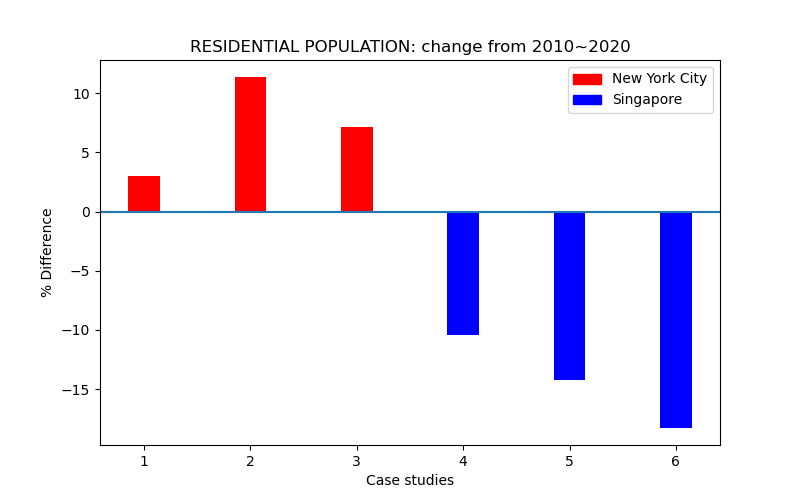
\includegraphics[width=0.5\textwidth]{Population_graph.png}
    \caption{\textbf{RESIDENTIAL POPULATION} Bar graph of residential population change of New York City vs Singapore 2010 ~ 2020}
\end{figure}


\begin{table}[H] 
    \centering
    \large
    \caption{New York City: Income change 2010 ~ 2020}

	\begin{tabular}{lccc}
		\hline
		New York City & West Village & BS and CH & OB and FR\\
		 & (\$) & (\$) & (\$)\\
		\hline
		2010 & 102,747 & 40,174 & 38,415\\
		2020 & 136,154 & 77,343 & 52,605\\
	    \% change & +24.54 & + 48.06 & +26.97\\
		\hline
	\end{tabular}
\end{table}

\begin{table}[H] 
    \centering
    \large
    \caption{Singapore: Income change 2010 ~ 2020}

    \begin{tabular}{lccc} 
		\hline
		Singapore & Ang Mo Kio & Bukit Merah & Gayland\\
		 & (\$) & (\$) & (\$)\\
		\hline
		2010 & 70,824 & 77,520 & 68,736\\
		2020 & 119,976 & 136,128 & 112,884\\
	    \% change & +40.96 & +43.06 & +39.11\\
		\hline
	\end{tabular}
\end{table}

\begin{figure}[H]
	\centering
	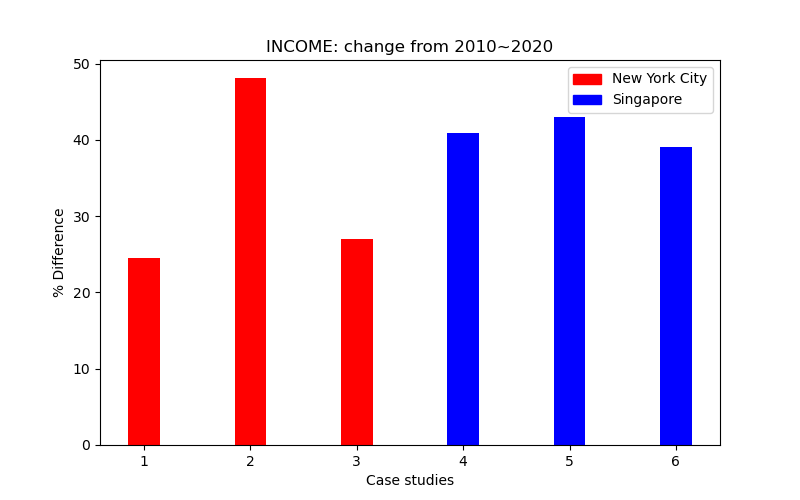
\includegraphics[width=0.5\textwidth]{Income_graph.png}
    \caption{\textbf{INCOME} Bar graph of income change of New York City vs Singapore 2010 ~ 2020}
\end{figure}

H-value of population: 3.857142857142854 \\
P-value: 0.049534613435626915 \\
H-value of income: 0.42857142857142705 \\
P-value: 0.5126907602619241 \\

With $\alpha$-value = 0.10, because the p-value of the population is less than $\alpha$ Kruskal-Wallis test does detect statistically significant differences for that group, however the p-value of the income is greater than $\alpha$ thus that group does not demonstrate sufficient statistical significance. The higher the h-value, the more different the groups are, therefore the h-value of population and income exhibits variation between the case studies of New York City and Singapore. \\

\subsection*{3.2 Literature analysis of Global North vs South vs East} 

\caption{\textbf{Literary Analysis of Gentrification Mechanisms: Global North vs South vs East}}
		Lists all 30 literary articles by order of Global North 1 ~ 10, Global South 11 ~ 20, Global East 21 ~ 30. Each article has listed the number of keywords detected out of the total per keyword bank for the theme of market-driven gentrification and theme of tenure-conversion gentrification. The overall theme of the article is chosen and listed in column 4 under "mechanism" based off the results of the keyword detection.}

\newpage

\begin{table}[H]
    \centering
    \footnotesize
	
	\begin{tabular}{lccc} 
		\hline
		Journal article \# & Market & Tenure & Mechanism\\
		  & (/22) & (/19) & \\
		\hline
        1 & 4 & 0 & Market\\
        2 & 5 & 2 & Market\\
        3 & 5 & 3 & Both\\
        4 & 3 & 2 & Neither\\
        5 & 5 & 1 & Market\\
        6 & 4 & 1 & Market\\
        7 & 3 & 1 & Neither\\
        8 & 2 & 1 & Neither\\
        9 & 5 & 2 & Market\\
        10 & 5 & 5 & Both\\
        11 & 4 & 5 & Both\\
        12 & 3 & 2 & Neither\\
        13 & 4 & 0 & Market\\
        14 & 2 & 2 & Neither\\
        15 & 3 & 1 & Neither\\
        16 & 5 & 3 & Both\\
        17 & 5 & 2 & Market\\
        18 & 7 & 4 & Both\\
        19 & 2 & 1 & Neither\\
        20 & 4 & 2 & Market\\
        21 & 2 & 3 & Tenure\\
        22 & 1 & 2 & Neither\\
        23 & 1 & 2 & Neither\\
        24 & 6 & 1 & Market\\
        25 & 2 & 0 & Neither\\
        26 & 2 & 6 & Tenure\\
        27 & 2 & 3 & Tenure\\
        28 & 7 & 3 & Both\\
        29 & 4 & 0 & Market\\
        30 & 2 & 3 & Tenure\\
		\hline
	\end{tabular}
\end{table}

\begin{figure}[H]
	\centering
	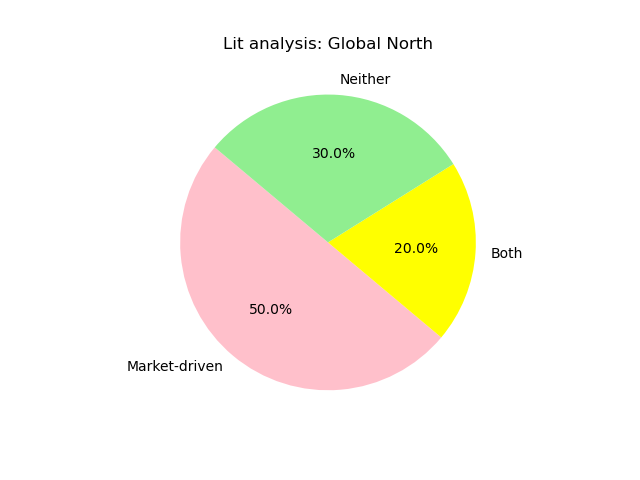
\includegraphics[width=0.5\textwidth]{North.png}
    \caption{\textbf{Global North} Pie chart for literary analysis. Breakdown of the different gentrification mechanisms attributed by each of the 10 articles pertaining to the Global North} 
\end{figure}

\begin{figure}[H]
	\centering
	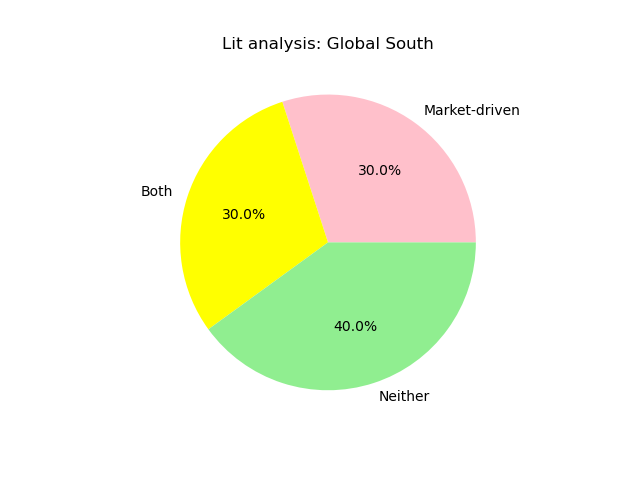
\includegraphics[width=0.5\textwidth]{South.png}
    \caption{\textbf{Global South} Pie chart for literary analysis. Breakdown of the different gentrification mechanisms attributed by each of the 10 articles pertaining to the Global North} 
\end{figure}

\begin{figure}[H]
	\centering
	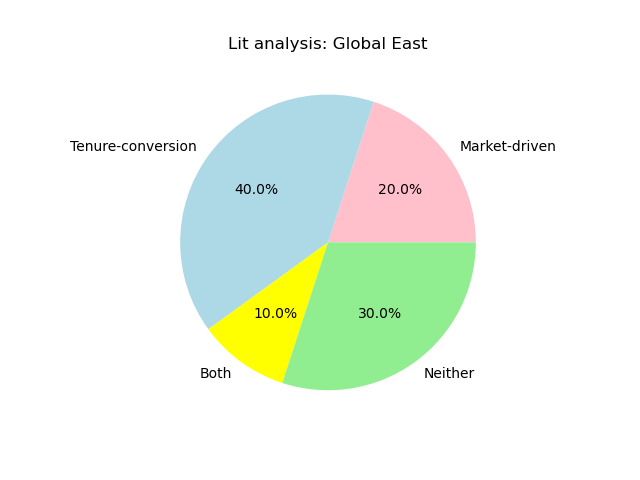
\includegraphics[width=0.5\textwidth]{East.png}
    \caption{\textbf{Global East} Pie chart for literary analysis. Breakdown of the different gentrification mechanisms attributed by each of the 10 articles pertaining to the Global North} 
\end{figure}

H-value of market-driven: 4.229503249767867 \\
P-value: 0.12066325558170642 \\
H-value of tenure-conversion: 0.8938216709571822 \\
P-value: 0.6396009354436645 \\

With $\alpha$-value = 0.10 both p-values are greater than $\alpha$ thus the Kruskal-Wallis test did not detect statistically significant differences. The higher the h-value, the more different the groups are, therefore the h-value of market-driven exhibits some variation among the Global North and Global South and Global East, whereas the h-value of tenure-conversion does not exhibit sufficient variation. \\


\section*{4 Conclusion}
This study observed and quantified differences in the effects of varied mechanisms of gentrification in the setting of global regions. However, there were a few limitations of the study which include. 1) Small sample size of the number of city case-studies and articles pulled, which limited the range of statistical analysis. 2) Inability to completely isolate variables such as income, residential populations, and mechanisms of gentrification, to determine the true cause of changes and indistinguishable regional variation factors. 3) Skewed spread of journal articles that were picked based on the content’s regional focus on the Global North or South or East but limited in the diversity of author and publisher backgrounds. \\

In the future, to solidify the study’s findings, a larger sample size and more complexly layered variables will be employed. With that stated, this study did contribute a representative understanding of global gentrification by visualizing the diversity in regional dependence of the causes and effects of gentrification. \\
	
The city case-studies showed that the two main mechanisms of gentrification, market-driven and tenure-conversion may have different effects in and of themselves depending on regionally specific factors and tenure systems. The literature analysis served as a semi-accurate model of detecting gentrification themes from journal articles. The quantitative results of the Global North, that 50\% of the articles expressed themes of market-driven gentrification, matched up with the qualitative research that rent-gap drives the competitive real estate market of the Global North. The Global South was split between articles on just market-driven, both market-driven and tenure-conversion, and neither, with the section of neither being the majority at 40\%. Gentrification in the Global South may not fall into either of the two themes due to different underlying contexts and mechanisms that did not exist within the list of keywords. The results of the Global East exhibited 40\% tenure-conversion and aligned with the Global East’s characteristic of heavy state involvement in housing. The model accurately identified that global regions exhibit different gentrification mechanisms, and as the city case-studies demonstrated, each of the mechanisms lead to different effects based on city factors. \\

Global gentrification involves various mechanisms and effects. Thus a single framework, specifically the dominant Anglo-American framework of gentrification, cannot be employed due to its inability to account for regional distinction and encapsulate the different causes and effects of gentrification worldwide. Gentrification must be placed in the context of the diversity of distinct regional attributes and tenure systems. \\

Further analysis could include looking into applying a case-study or literary-analysis approach in disproving diffusion theory that gentrification diffused from the Global North to the Global South and Global East, and or researching more similarities and differences of global gentrification, thus revolutionizing the framework from which global gentrification is considered. \\

\section*{5 Acknowledgments}
I would like to thank my mentor, June Postalakis, for supporting and inspiring me. Through her sharing her knowledge in her field of work, brainstorming research topics with me, and kindly answering my many questions, she has guided me on my journey to develop a research project. I am forever grateful for her generosity and dedicate my newfound love of research to her. I would also like to thank Dr. Mark Galassi for teaching me skills in coding, research, and critical thinking. And I would like to thank Doug Mandell and Karen for supporting us Portland interns through this process. Most of all I truly appreciate the Institute for providing me with this opportunity to explore the field of research.\\

\section*{6 References}
\nocite{*}
\printbibliography[heading=none]

\end{document}
